% Created:  
% Author:   Julie Sewards
% Filename: implementation.tex

\chapter{Implementation}
\label{cha:imp}
\section{Development Environment}
An early challenge encountered in this project was setting up a suitable development environment.  Initially the intention was to use the Android Development Tools plug-in for Eclipse, as this was an extension to an already familiar IDE, however, difficukties were encoulntered with the school computers and finally we elected to switch to Android Studio (Beta) as suggested on the Android Developers website \cite{android_dev}.  

Since the main rationale for the Android application was to allow users to read documents away fro the PC, we felt that the application should be optimised for use on a tablet.  As difficulty was encountered getting the device emulators to work on Linux, it became necessary to purchase a physical device for the purposes of the project.  As budget was a significant consideration, the device chosen was a Hudl 7" tablet running the Android 4.2.2 Jelly Bean operating system.  For the purposes of this project, it was decided that we would develop and test for this device.  This meant that we were restricted to API 17, which eliminated the need to include any backward compatibility but also precluded using features of the latest Android releases as it transpired that there was no upgrade path available for this device.  This fact turned out to be highly significant in a later stage of the project.  

\section{Initial Development}
As we had no previous experience of developing for the Android platform, it was felt wise to develop a very simple application in order to gain some familiarity with the complexities of the Android architecture and its API. This initial application enabled us to input some text, encrypt it (using a simple "convert to upper case" as a place-holder for encryption) and write it to the application storage.  

The next stage was to introduce real encryption, for which we needed to investigate the Java Cryptography Architecture(JCA).  Although the choice of algorithm was determined as part of the design, we were mindful of the fact that  many security weaknesses are introduced by poor implementation. As \citet{schneier1998security} states,
\begin{quotation}
And just as it's possible to build a weak structure using strong materials, it's possible to build a weak cryptographic system using strong algorithms and protocols 
\end{quotation}  
For this reason we decided that we would initially develop and test the  Java classes to be used for encryption and decryption in the more familiar Linux environment before porting to Android.  Linux also provides a simple command line interface which was valuable for inspecting the binary (or hex) content of encrypted files to aid debugging.


/red {I am still tidying up from here on - have just left headers as placeholders for now}\\


\section{SecurelyShare Prototype}

In order to widen our experience of Android development, we sought to include a variety of different techniques

\begin{figure}[h!]
    \centering
    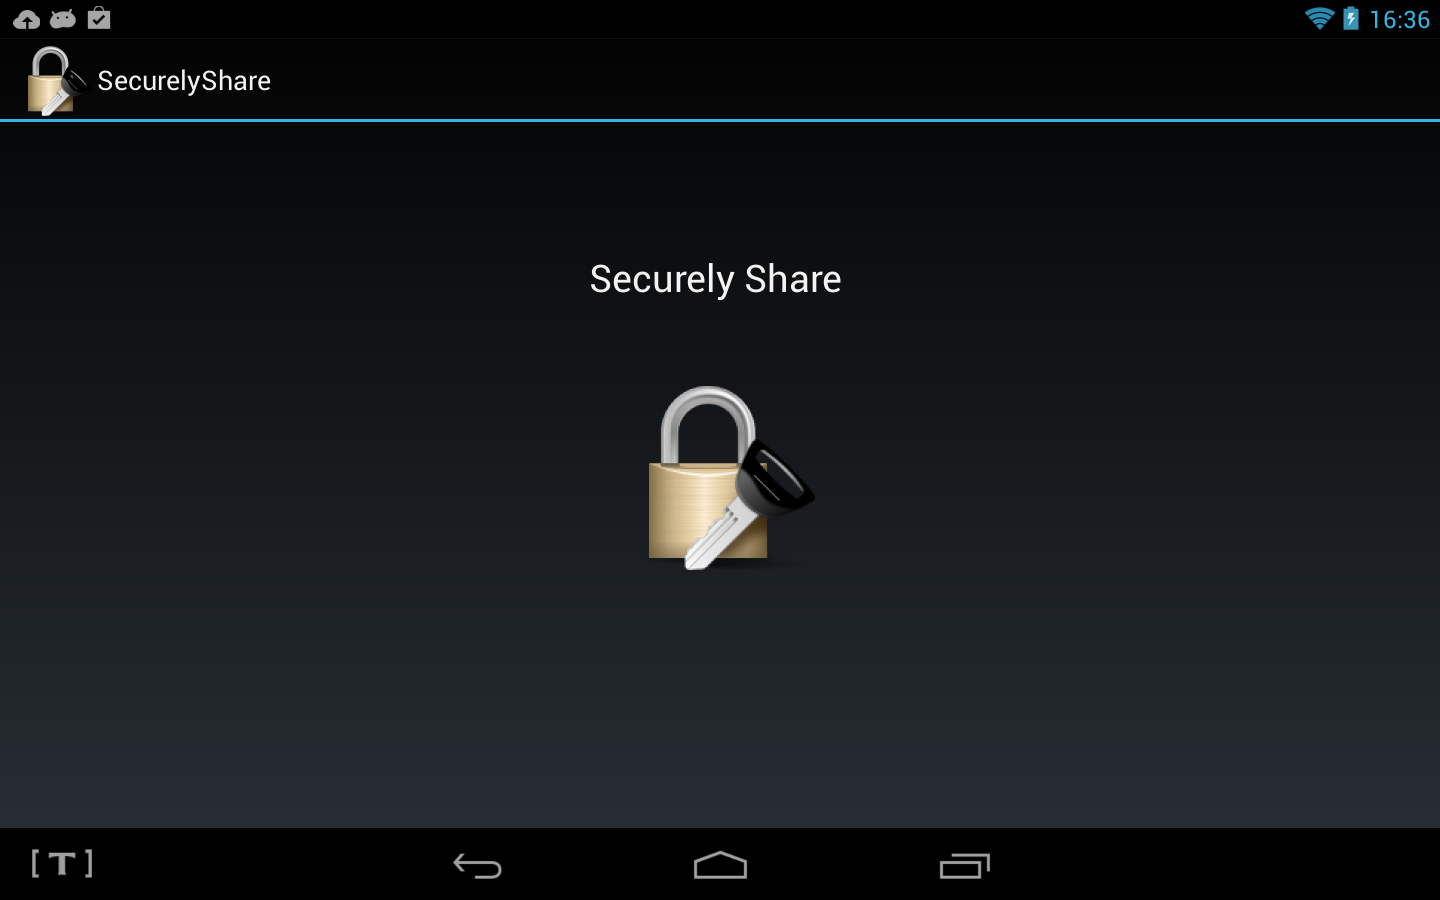
\includegraphics[width=0.4\textwidth]{SplashScreen}
    \caption{Initial splash screen }
    \label{fig:initial}
\end{figure}


\begin{figure}[h!]
    \centering
    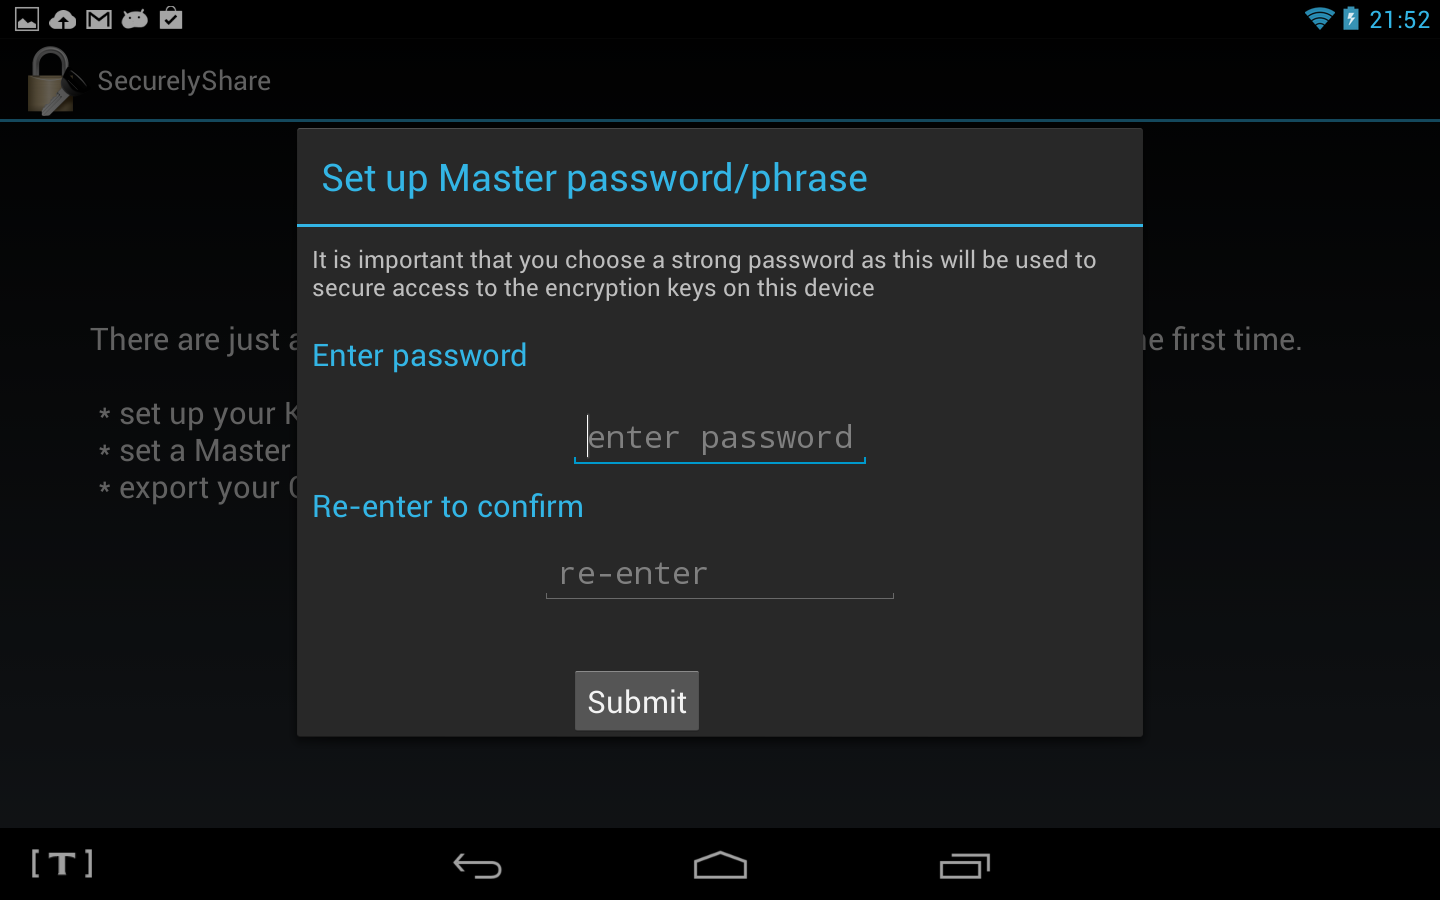
\includegraphics[width=0.4\textwidth]{Setup}                                                                                                                                                                                                                                                                                                                                                                                                                                                                                                                                                                                                                                                                                                                                                                                                                                                                                                                                                                                                                                                                                                                                                                                                                                                                                                                                                                                                                                                                                                                                                                                                                                                                                                                                                                                                                                                                                                                                                                                                                                                                                                                                                                                                                                                                                                                                                                                                                                                                                                                                                                                                                                                                                                                                                                                                                                                                                                                                                                          
    \caption{Setup Master Password }
    \label{fig:alert}
\end{figure}
\section{Implementation Challenges}
\section{Testing}

\chapter{Project Management}
\chapter{Evaluation}
\section{Security Evaluation}
\section{Product Evaluation}
\section{Process Evaluation}
As outlined in the Introduction, one of our goals in yundertaking this projhect was to gain some experience of development for the Android platform and as such it was important that we aspired to seek out and use 'best practice' wherever possible.  
\section{Future Work}
\chapter{Conclusion}


